\section{Experiments}
\label{sec:exp}

\subsection{Setup}
\label{sec:setup}

\paragraph{Data.}
We use only the official Hugging Face PushT expert release
(\texttt{quentinll/lewm-pusht}, HDF5).
A reproducible subset of \textbf{1000} windows is drawn with seed
\textbf{3072} and split by \texttt{spt.random\_split([0.9, 0.1])} into
\textbf{901} train / \textbf{99} validation windows
(indices frozen; never regenerated between runs).
Of the 99 val windows, \textbf{93} remain feasible under
\texttt{goal\_offset=25} for CEM (6 dropped).

\paragraph{Models and compute.}
Both predictors use ViT-tiny, history 3, $D{=}192$, SIGReg
$\lambda{=}0.09$, AdamW lr $5{\times}10^{-5}$, weight decay
$10^{-3}$, grad clip 1.0, bf16, 100 epochs, frameskip 5.
Hardware: RTX~4060 Laptop (8\,GiB); batch 64 with gradient
accumulation 2 (effective 128); \texttt{num\_workers=0}.
Parameter counts: discrete AR \textbf{18,034,478}; ODE
\textbf{18,071,534} (+37,056 from $v$-head).

\begin{table}[t]
\centering
\caption{Experimental setup (PushT 1k subset).}
\label{tab:setup}
\begin{tabular}{lc}
\toprule
Item & Value \\
\midrule
Dataset & Official HF PushT expert HDF5 \\
Subset / seed & 1000 windows / 3072 \\
Train / val & 901 / 99 \\
CEM eval set & val-99 $\to$ 93 feasible \\
Encoder & ViT-tiny, patch 14, $224^2$, scratch \\
SIGReg & $\lambda{=}0.09$, $M{=}1024$, knots 17 \\
ODE solver & RK4, $N{=}4$, $\tau{:}0\to1$ \\
Params (ODE) & 18,071,534 ($\approx$18.07M) \\
Train & 100 epochs, AdamW $5{\times}10^{-5}$ \\
Effective batch & 128 (64$\times$accum~2) \\
\bottomrule
\end{tabular}
\end{table}

\subsection{Results}
\label{sec:results}

\begin{table}[t]
\centering
\caption{PushT 1k$\times$100ep: loss and CEM (same split).
Paper PushT success is under full-data training, shown for context only.}
\label{tab:results}
\begin{tabular}{lcccc}
\toprule
Method & Params & fit/loss & val/loss & CEM val-99 \\
\midrule
Discrete AR (\LeWM{}) & 18.03M & 0.248 & 0.536 & 5/93 (5.38\%) \\
ODE RK4 0$\to$1 (ours) & 18.07M & \textbf{0.234} & \textbf{0.506} & 5/93 (5.38\%) \\
\midrule
\LeWM{} paper (full data) & $\sim$15M & --- & --- & $96{\pm}2.83$\%$^\dagger$ \\
\bottomrule
\multicolumn{5}{l}{\footnotesize $^\dagger$Reported PushT success; not comparable to our 1k protocol.} \\
\end{tabular}
\end{table}

\begin{figure}[t]
\centering
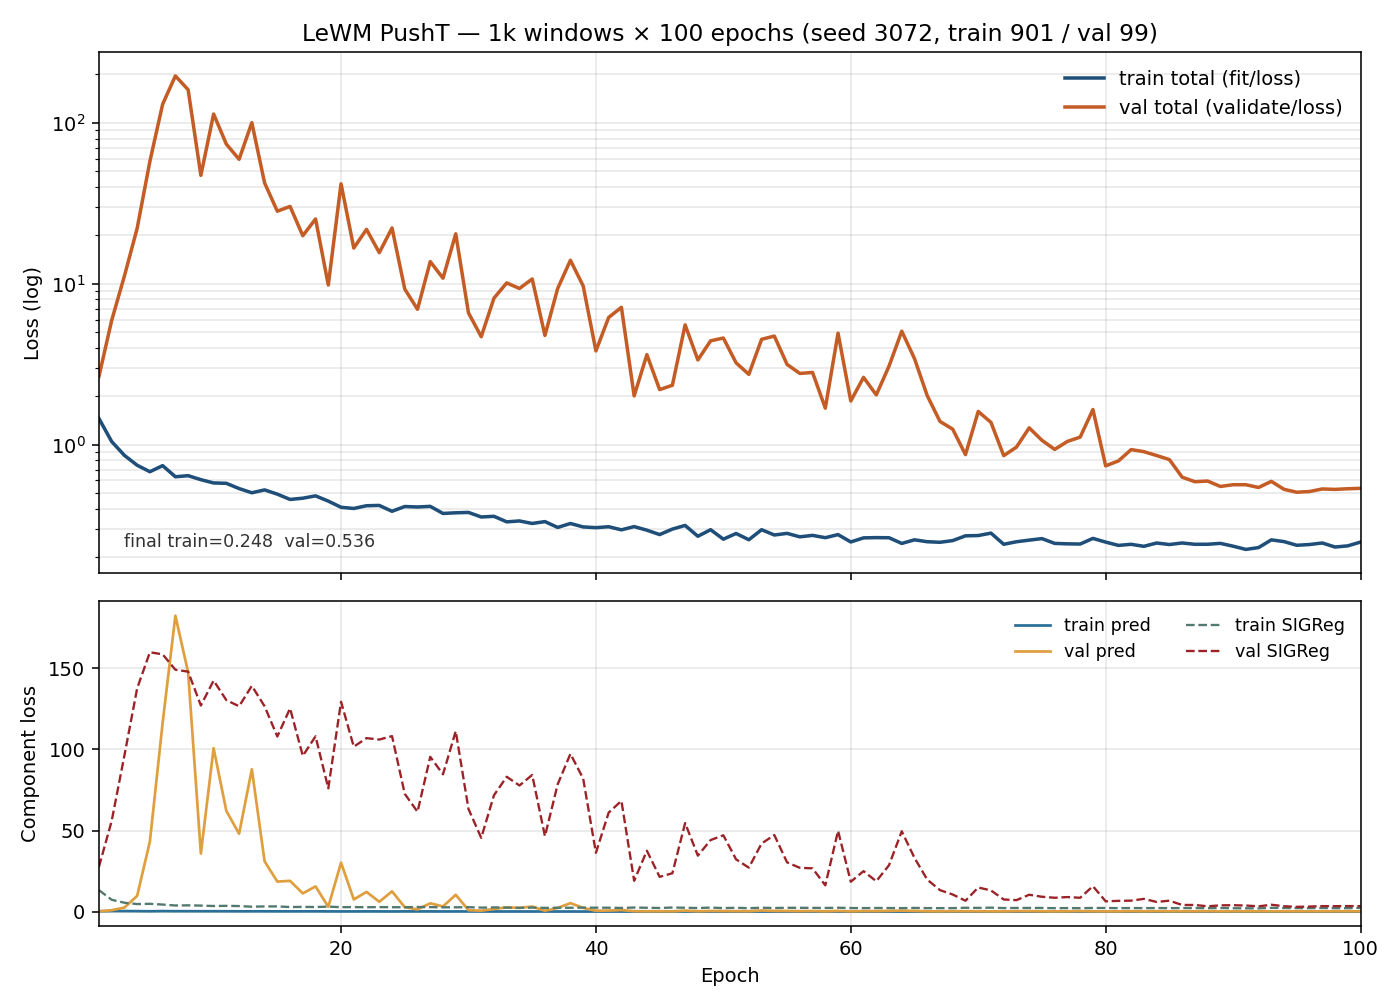
\includegraphics[width=0.48\linewidth]{figs/lewm_train_loss.png}%
\hfill
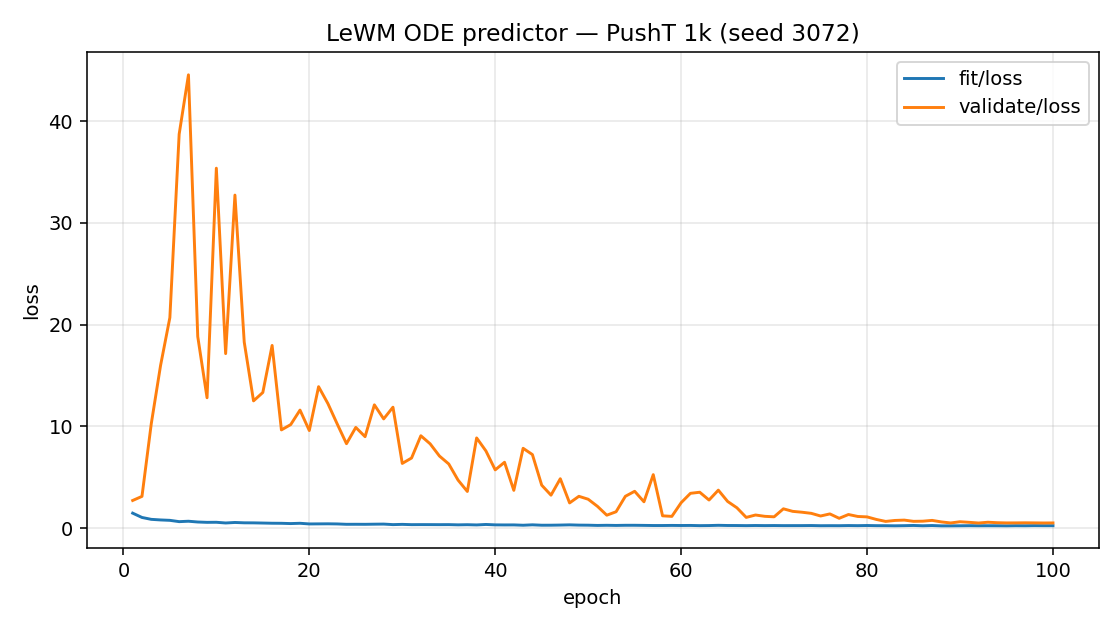
\includegraphics[width=0.48\linewidth]{figs/lewm_ode_train_loss.png}
\caption{Training curves on the fixed 1k split (left: discrete AR;
right: ODE predictor). ODE converges to lower fit/val loss.}
\label{fig:curves}
\end{figure}

Table~\ref{tab:results} summarizes the matched comparison.
The ODE predictor improves fit/loss (0.234 vs.\ 0.248) and val/loss
(0.506 vs.\ 0.536); final val prediction / SIGReg terms are
approximately 0.220 / 3.17.
CEM success is identical: \textbf{5 successes out of 93} feasible
val starts ($\approx$5.38\%).
ODE CEM wall-clock is substantially higher ($\approx$82\,min vs.\
$\approx$8\,min for discrete on the same machine) because each
rollout step runs four RK4 stages.

\paragraph{Protocol note.}
Earlier CEM probes on random full-dataset starts (e.g.\ 0/10) are
\emph{not} val-tied and are discarded; all claims here use the
val-99 / 93-feasible protocol shared with \texttt{validate/loss}.

\subsection{Limitations}
\label{sec:limitations}

\begin{itemize}[leftmargin=*,itemsep=2pt]
\item \textbf{1k subset.} Results are on 1000 windows, not the full
PushT expert corpus. Paper-scale $\approx$96\% success is out of
scope for this study.
\item \textbf{CEM tied.} Lower loss does not yield higher CEM success
under this budget; planning may be bottlenecked by data scale, CEM
hyperparameters, or goal-offset feasibility rather than predictor
form.
\item \textbf{Single environment.} Only PushT is evaluated; Cube,
Two-rooms, and Reacher remain future work.
\item \textbf{Fixed solver.} We use RK4 with $N{=}4$ and no adaptive
stepping; broader ODE solvers and multi-step $\tau$ schedules are
unexplored.
\end{itemize}
